% \documentclass[draft,11pt]{article}
\chapter{Some Basic Optimization, Convex Geometry, and
  Linear Algebra}
\label{sec:cvopt}

%%% for this lecture

%\begin{document}
\sloppy
%\lecture{2 --- Wednesday, February 26}
%{Spring 2020}{Rasmus Kyng}{Some Basic Optimization, Convex Geometry, and
  %Linear Algebra}

\section{Overview}

In this chapter, we will

\begin{enumerate}
\item Start with an overview (i.e. this list).
\item Learn some basic terminology and facts about optimization.
\item Recall our definition of convex functions and see how
  convex functions can also be understood in terms of a
  characterization based on first derivatives.
\item See how the first derivatives of a convex function can certify
  that we are at a global minimum.
\end{enumerate}


\section{Optimization Problems}
Focusing for now on optimization over $\xx \in \R^n$, we usually write optimization problems as:
\begin{align*}
\min_{\xx \in \R^n} \ ( \textrm{or} \ \max) & \ f(\xx)\\
s.t. & \ g_1(\xx) \leq b_1 \\
	& \ . \\
	& \ . \\
	& \ . \\
	& \ g_m(\xx) \leq b_m  \label{cond1}
%
\end{align*}
%
where $\{g_{i}(\xx)\}_{i=1}^{m}$ encode the constraints. For example, in the following optimization problem from the previous chapter
\begin{align*}
\min_{\ff \in \R^E} & \sum_e \rr(e) \ff(e)^2 \\
\textrm{s.t. } & \BB \ff = \dd
\end{align*}
we have the constraint $\BB \ff = \dd$. Notice that we can rewrite this constraint as $\BB \ff \le \dd$ and $-\BB \ff \le -\dd$ to match the above setting.\ The set of points which respect the constraints is called the \emph{feasible set}.

\boxdef{For a given optimization problem the set $\mathcal{F}=\{\xx
  \in \R^n \ : \ g_{i}(\xx) \leq b_i, \forall i \in [m]\}$ is called
  the \textbf{feasible set}.  A point $\xx \in \mathcal{F}$ is called
  a \textbf{feasible point}, and a point $\xx' \notin \mathcal{F}$ is called an \textbf{infeasible point}.}

Ideally, we would like to find optimal solutions for the optimization problems we consider.  Let's define what we mean exactly.

\boxdef{
For a \emph{maximization} problem $\xx^\star$ is called an \textbf{optimal solution } if $f(\xx^\star) \geq f(\xx)$, $\forall \xx \in \mathcal{F}$.  Similarly, for a \emph{minimization} problem $\xx^\star$ is an optimal solution if $f(\xx^\star) \leq f(\xx)$, $\forall \xx \in \mathcal{F}$.
}

What happens if there are \emph{no feasible points}?
In this case, an optimal solution cannot exist, and we say the problem
is infeasible.

\boxdef{
If $\mathcal{F} = \emptyset$ we say that the optimization problem is \textbf{infeasible}.  If $\mathcal{F} \neq \emptyset$ we say the optimization problem is \textbf{feasible}.
}

\begin{figure}[h]
  \centering
     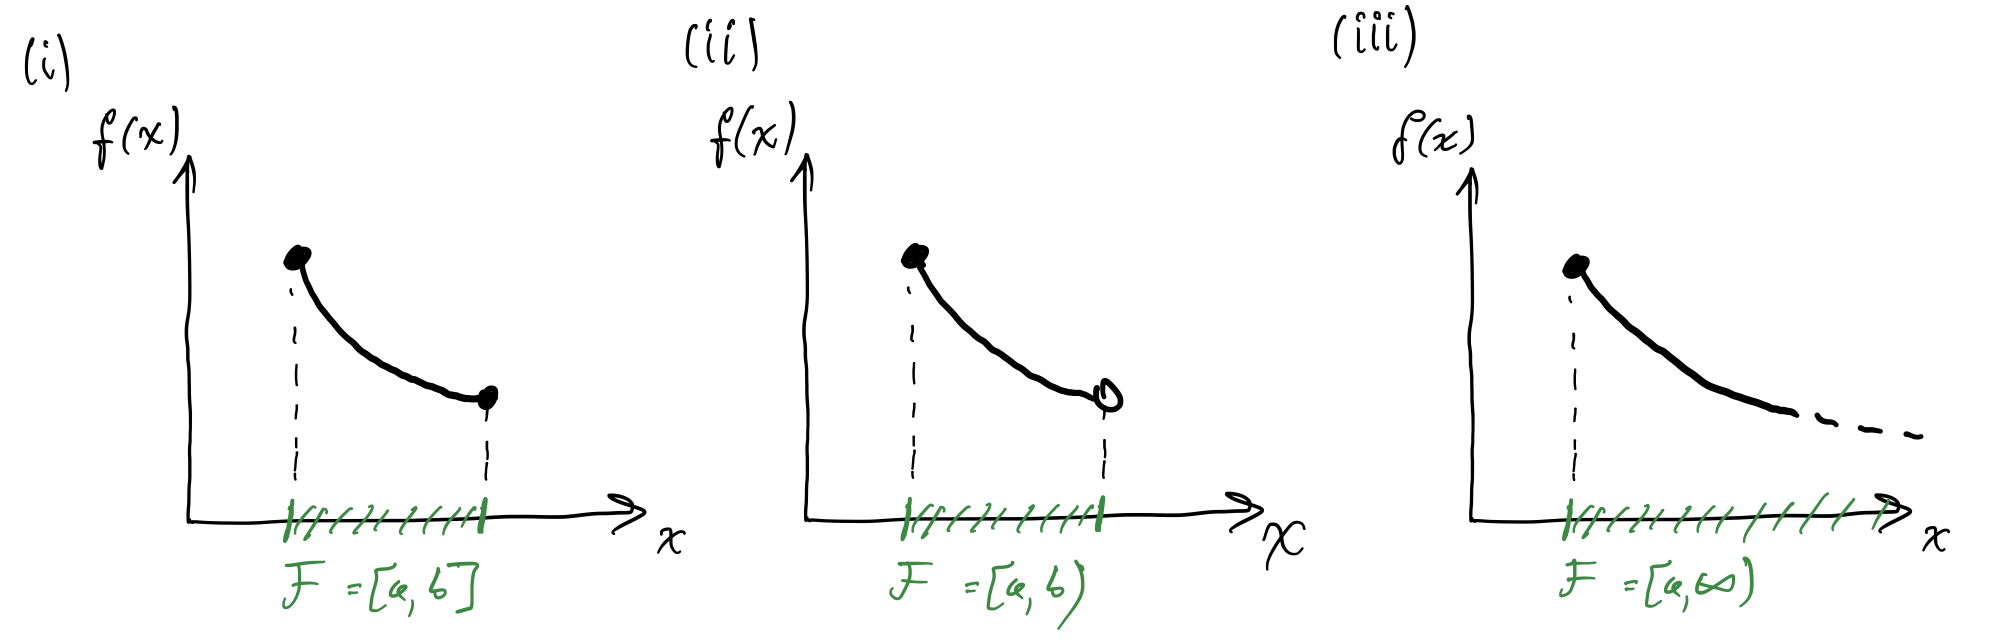
\includegraphics[width=\textwidth]{fig/lect1_attaining-min.png}
%                 \caption{
% \todo{!}
% }
\caption{}
\label{fig:regions}
\end{figure}

Consider three examples depicted in Figure 2.1:

\begin{enumerate}[label=(\roman*)]
\item $\mathcal{F} = [a,b]$
\item $\mathcal{F} = [a,b)$
\item $\mathcal{F} = [a,\infty)$
\end{enumerate}

In the first example, the minimum of the function is attained at $b$.
In the second case the region is open and therefore there is
no minimum function value, since for every point we will choose,
there will always be another point with a smaller function value.
Lastly, in the third example, the region is unbounded and the function
decreasing, thus again
there will always be another point with a smaller function value.




\paragraph{Sufficient Condition for Optimality.}
The following theorem, which is a fundamental theorem in real analysis, gives us a sufficient (though not necessary) condition for optimality.
\begin{theorem*}[Extreme Value Theorem]
Let $f:\mathbb{R}^n \to \mathbb{R}$ be a continuous function and $\mathcal{F} \subseteq \mathbb{R}^n$ be nonempty, bounded, and closed.  Then, the optimization problem $\min f(\xx) : \xx \in \mathcal{F}$ has an optimal solution.
\end{theorem*}

\section{A Characterization of Convex Functions}
Recall the definitions of convex sets and convex functions that we
introduced in Chapter~\ref{cha:intro}:

\boxdef{
A set $S \subseteq \R^n$ is called a \textbf{convex set} if any two points in $S$ contain their line, i.e. for any $\xx,\yy \in S$ we have that $\theta \xx + (1-\theta)\yy \in S$ for any $\theta \in [0,1]$.
}

\boxdef{
For a convex set $S \subseteq \R^n$, we say that a function $f:S \to \mathbb{R}$ is  \textbf{convex on $S$} if for any two points $\xx,\yy \in S$ and any $\theta \in [0,1]$ we have that:
%
$$ f\left (\theta \xx + (1-\theta)\yy \right ) \leq \theta f (\xx) + \Big (1-\theta\Big )f(\yy).$$
%
}


\begin{figure}[h]
  \centering
     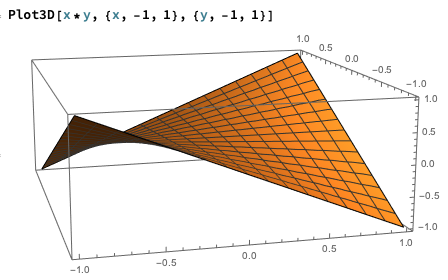
\includegraphics[width=0.4\textwidth]{fig/lecture2_plot3d-nonjointconvex.png}
\caption{This plot shows the function $f(x,y) = xy$. For any fixed
  $y_0$, the function $h(x) = f(x,y_0) = xy_0$ is
this is linear in $x$, and so is a convex
function in $x$. But is $f$ convex?}
\label{fig:nonjointconvex}
\end{figure}

We will first give an important characterization of convex function.  To do so, we need to characterize multivariate functions via their Taylor expansion.
%\subsection{First Order Taylor Expansion}

\paragraph{Notation for this section.}
  In the rest of this section, we frequently consider a multivariate functions $f$
  whose domain is a set $S \subseteq \R^n$, which we will require to
  be open.
  When we additionally require that $S$ is convex, we will specify this.
  Note that $S = \R^n$ is both open and convex and it suffices to keep
  this case in mind.
  Things sometimes get more complicated if $S$ is not open, e.g. when the
  domain of $f$ has a boundary.
  We will leave those complications for another time.

\subsection{First-order Taylor Approximation}

\boxdef{
%Let $S \subseteq \R^n$.
  The \textbf{gradient} of a function $f:S \to \R$ at point $\xx
  \in S$ is denoted $\grad f(\xx)$ is:
\begin{displaymath}
    \grad f(\xx) = \left[\frac{\partial f(\xx)}{\partial \xx(1)},\ldots, \frac{\partial f(\xx)}{\partial \xx(n)}\right]^\trp
\end{displaymath}
}
%
\paragraph{First-order Taylor expansion.}
For a function $f:\R\rightarrow\R$ of a single variable,
differentiable at $x \in \R$
\begin{displaymath}
    f(x+\delta) = f(x) + f'(x) \delta + o(\abs{\delta})
\end{displaymath}
where by definition:
\begin{displaymath}
    \lim_{\delta\rightarrow 0} \frac{o(\abs{\delta})}{\abs{\delta}} = 0
    .
  \end{displaymath}
  Similarly, a multivariate function $f:S \rightarrow \R$
  %, where $S \subseteq\R^n$,
  is said to
be
\emph{(Fr\'{e}chet) differentiable} at $\xx \in S$ when there exists
$\grad f(\xx) \in \R^n$ s.t.
\begin{displaymath}
  \lim_{\ddelta \to \veczero}
  \frac{\norm{f(\xx+\ddelta) - f(\xx) -\grad f(\xx)^{\trp} \ddelta  }_2}{
    \norm{\ddelta}_2
  } = 0
    .
\end{displaymath}
Note that this is equivalent to saying that
$f(\xx+\ddelta) = f(\xx) + \grad f(\xx)^\trp\ddelta +
o(\norm{\ddelta}_2)$.

We say that $f$ is \emph{continuously differentiable} on a set $S \subseteq \R^n $ if it is
differentiable and in addition the gradient is continuous on $S$.
A differentiable convex function whose domain is an
open convex set $S \subseteq \R^n $ is always continuously
differentiable\footnote{See p. 248, Corollary 25.5.1 in \emph{Convex
    Analysis} by Rockafellar (my version is the Second print,

  1972). Rockefellar's corollary concerns finite convex functions, because he
  otherwise allows convex functions that may take on the values $\pm \infty$. }.

\begin{remark*}
  In this course, we will generally err on the side of being informal
  about functional analysis when we can afford to, and we will not
  worry too much about the
  about details of different notions of differentiability
  (e.g. Fr\'{e}chet and Gateaux differentiability), except when
  it turns out to be important.
\end{remark*}

\begin{theorem}[Taylor's Theorem, multivariate first-order remainder form]
  If $f:S \rightarrow \R$
  %, where $S \subseteq \R^n$,
  is continuously differentiable over $[\xx, \yy]$, then for
  some $\zz \in [\xx, \yy]$,
\begin{displaymath}
    f(\yy) = f(\xx) + \grad f(\zz)^\trp (\yy-\xx).
\end{displaymath}
\end{theorem}

This theorem is useful for showing that the function $f$ can be
approximated by the affine function  ${\yy \to f(\xx) + \grad f(\xx)^\trp (\yy-\xx)}$
when $\yy$ is ``close to'' $\xx$ in some sense.

% \begin{figure}[!tbp]
%   \centering
%   \begin{minipage}[b]{0.45\textwidth}
%      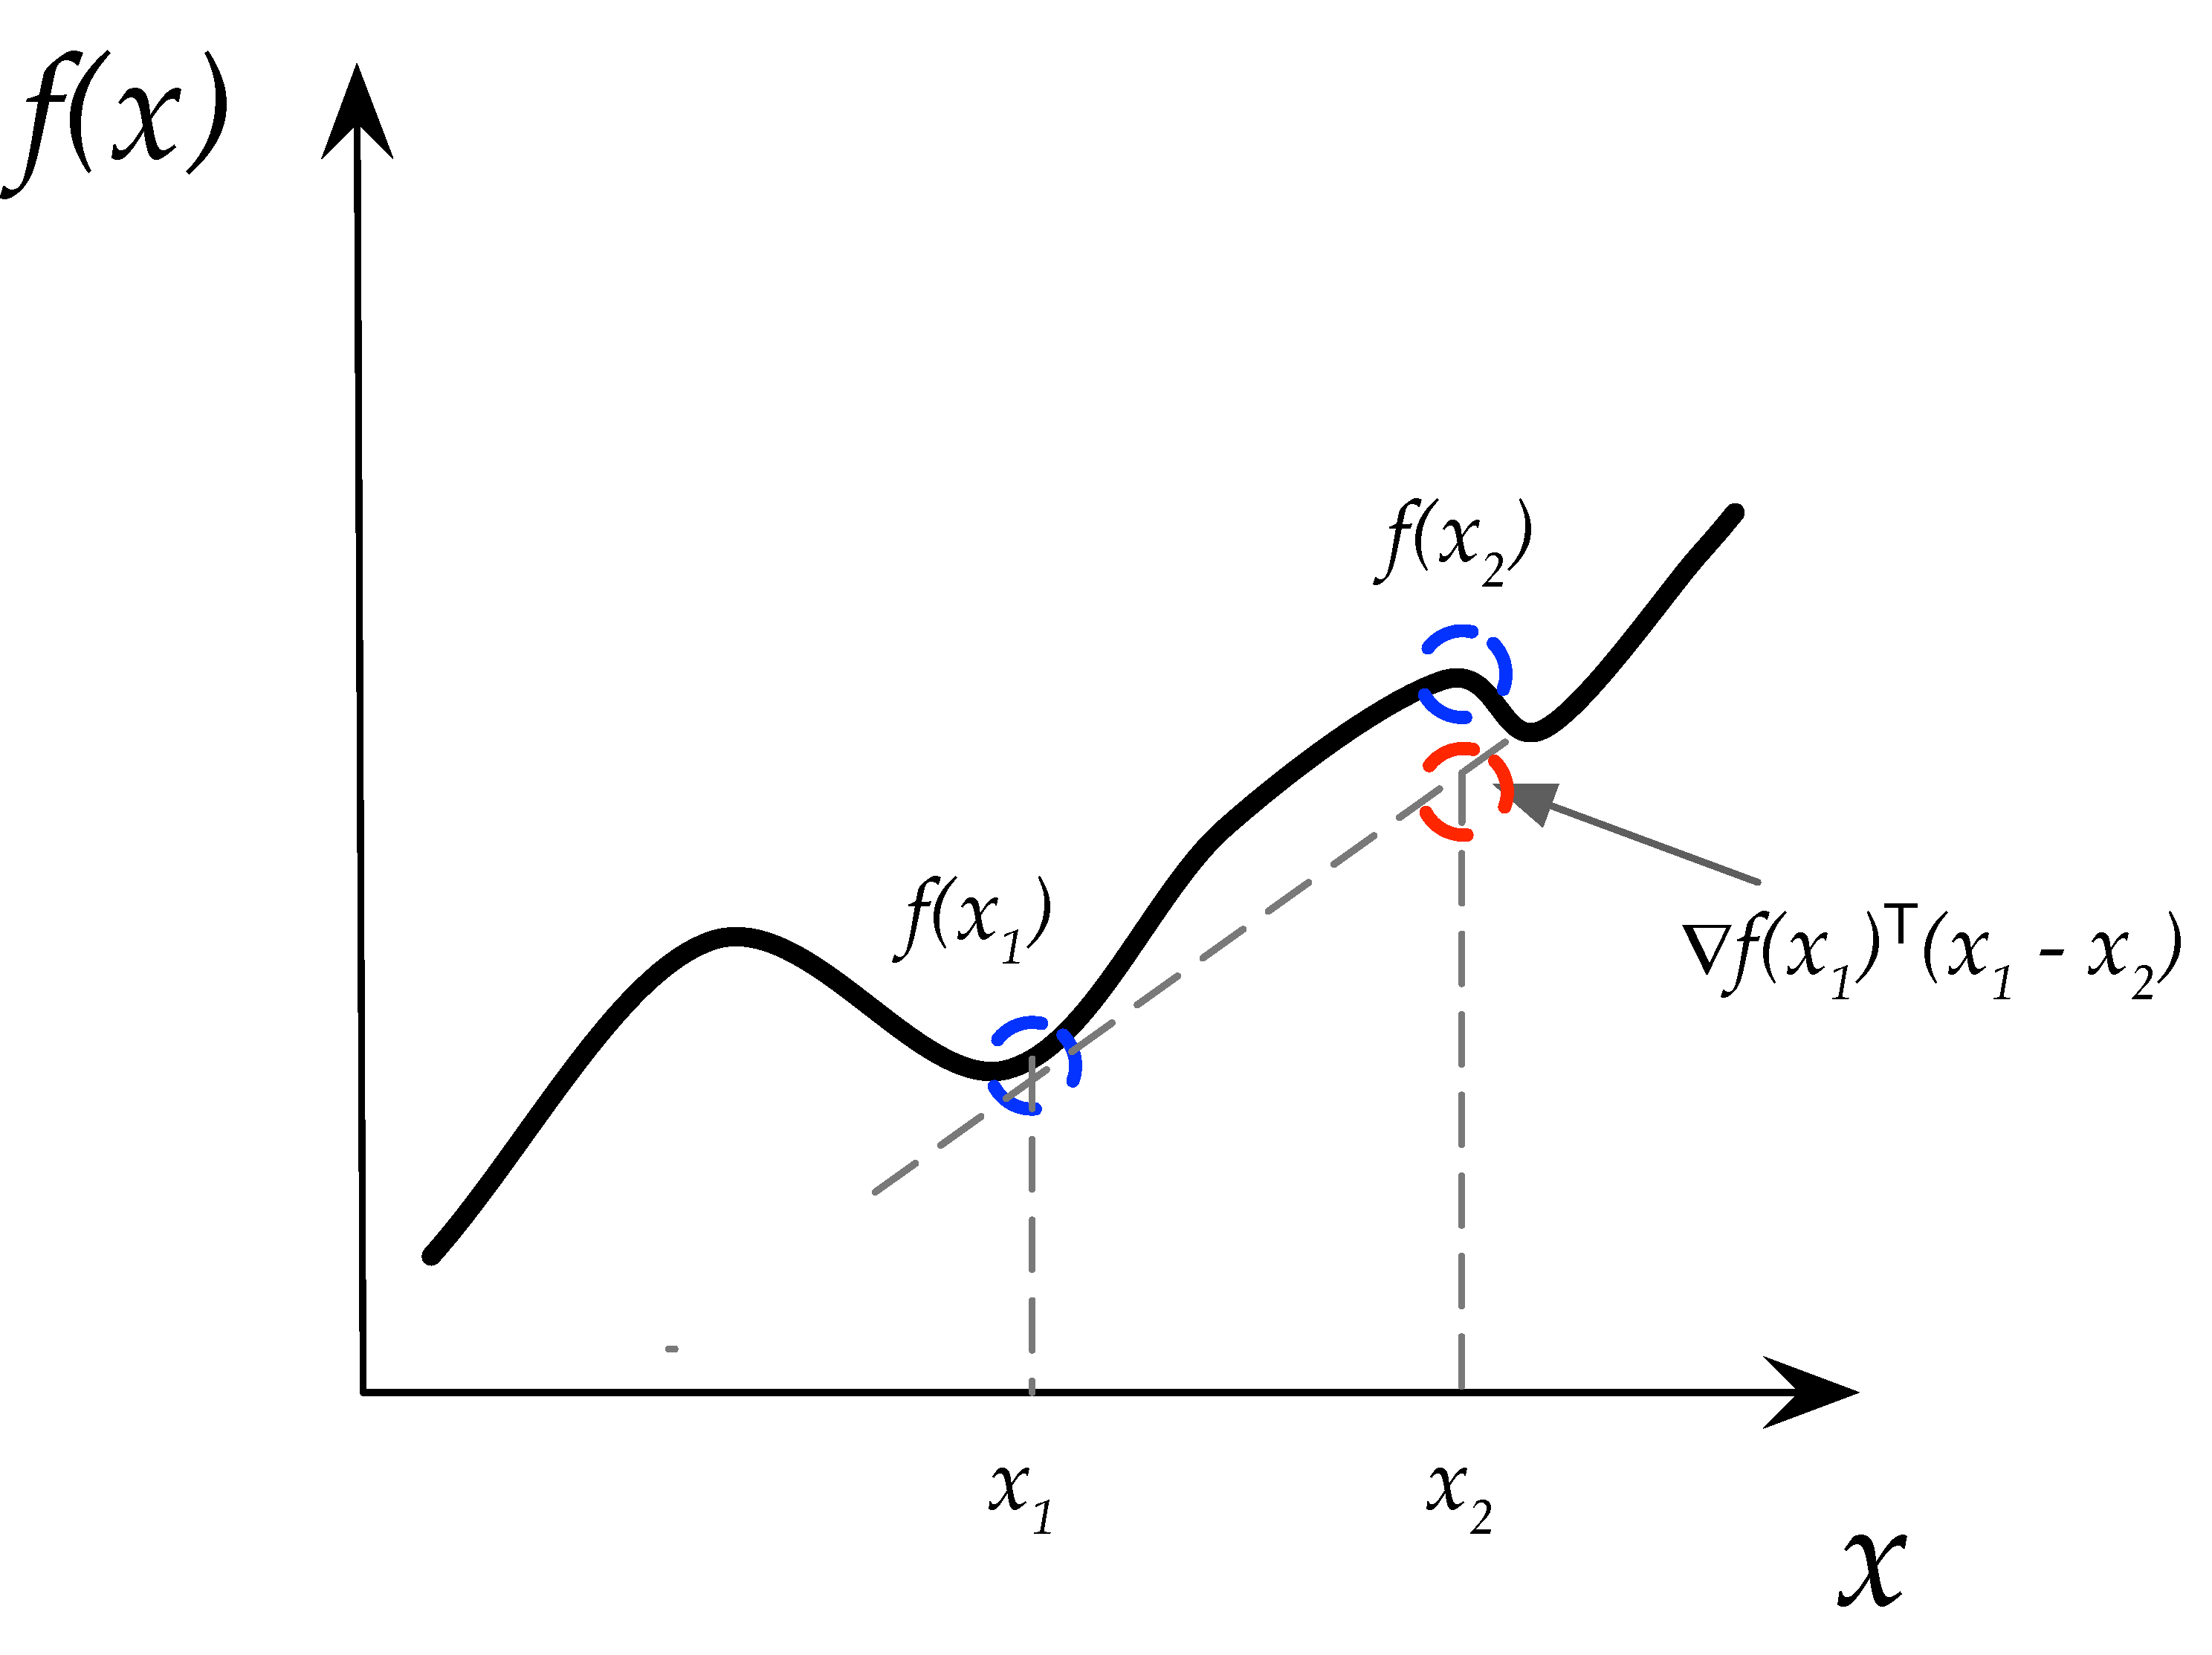
\includegraphics[trim = 0mm 0mm 0mm 0mm, height=60mm]{fig/lec8_taylor1.pdf}
%                    \end{minipage}
%   \hfill
%   \begin{minipage}[b]{0.45\textwidth}
%    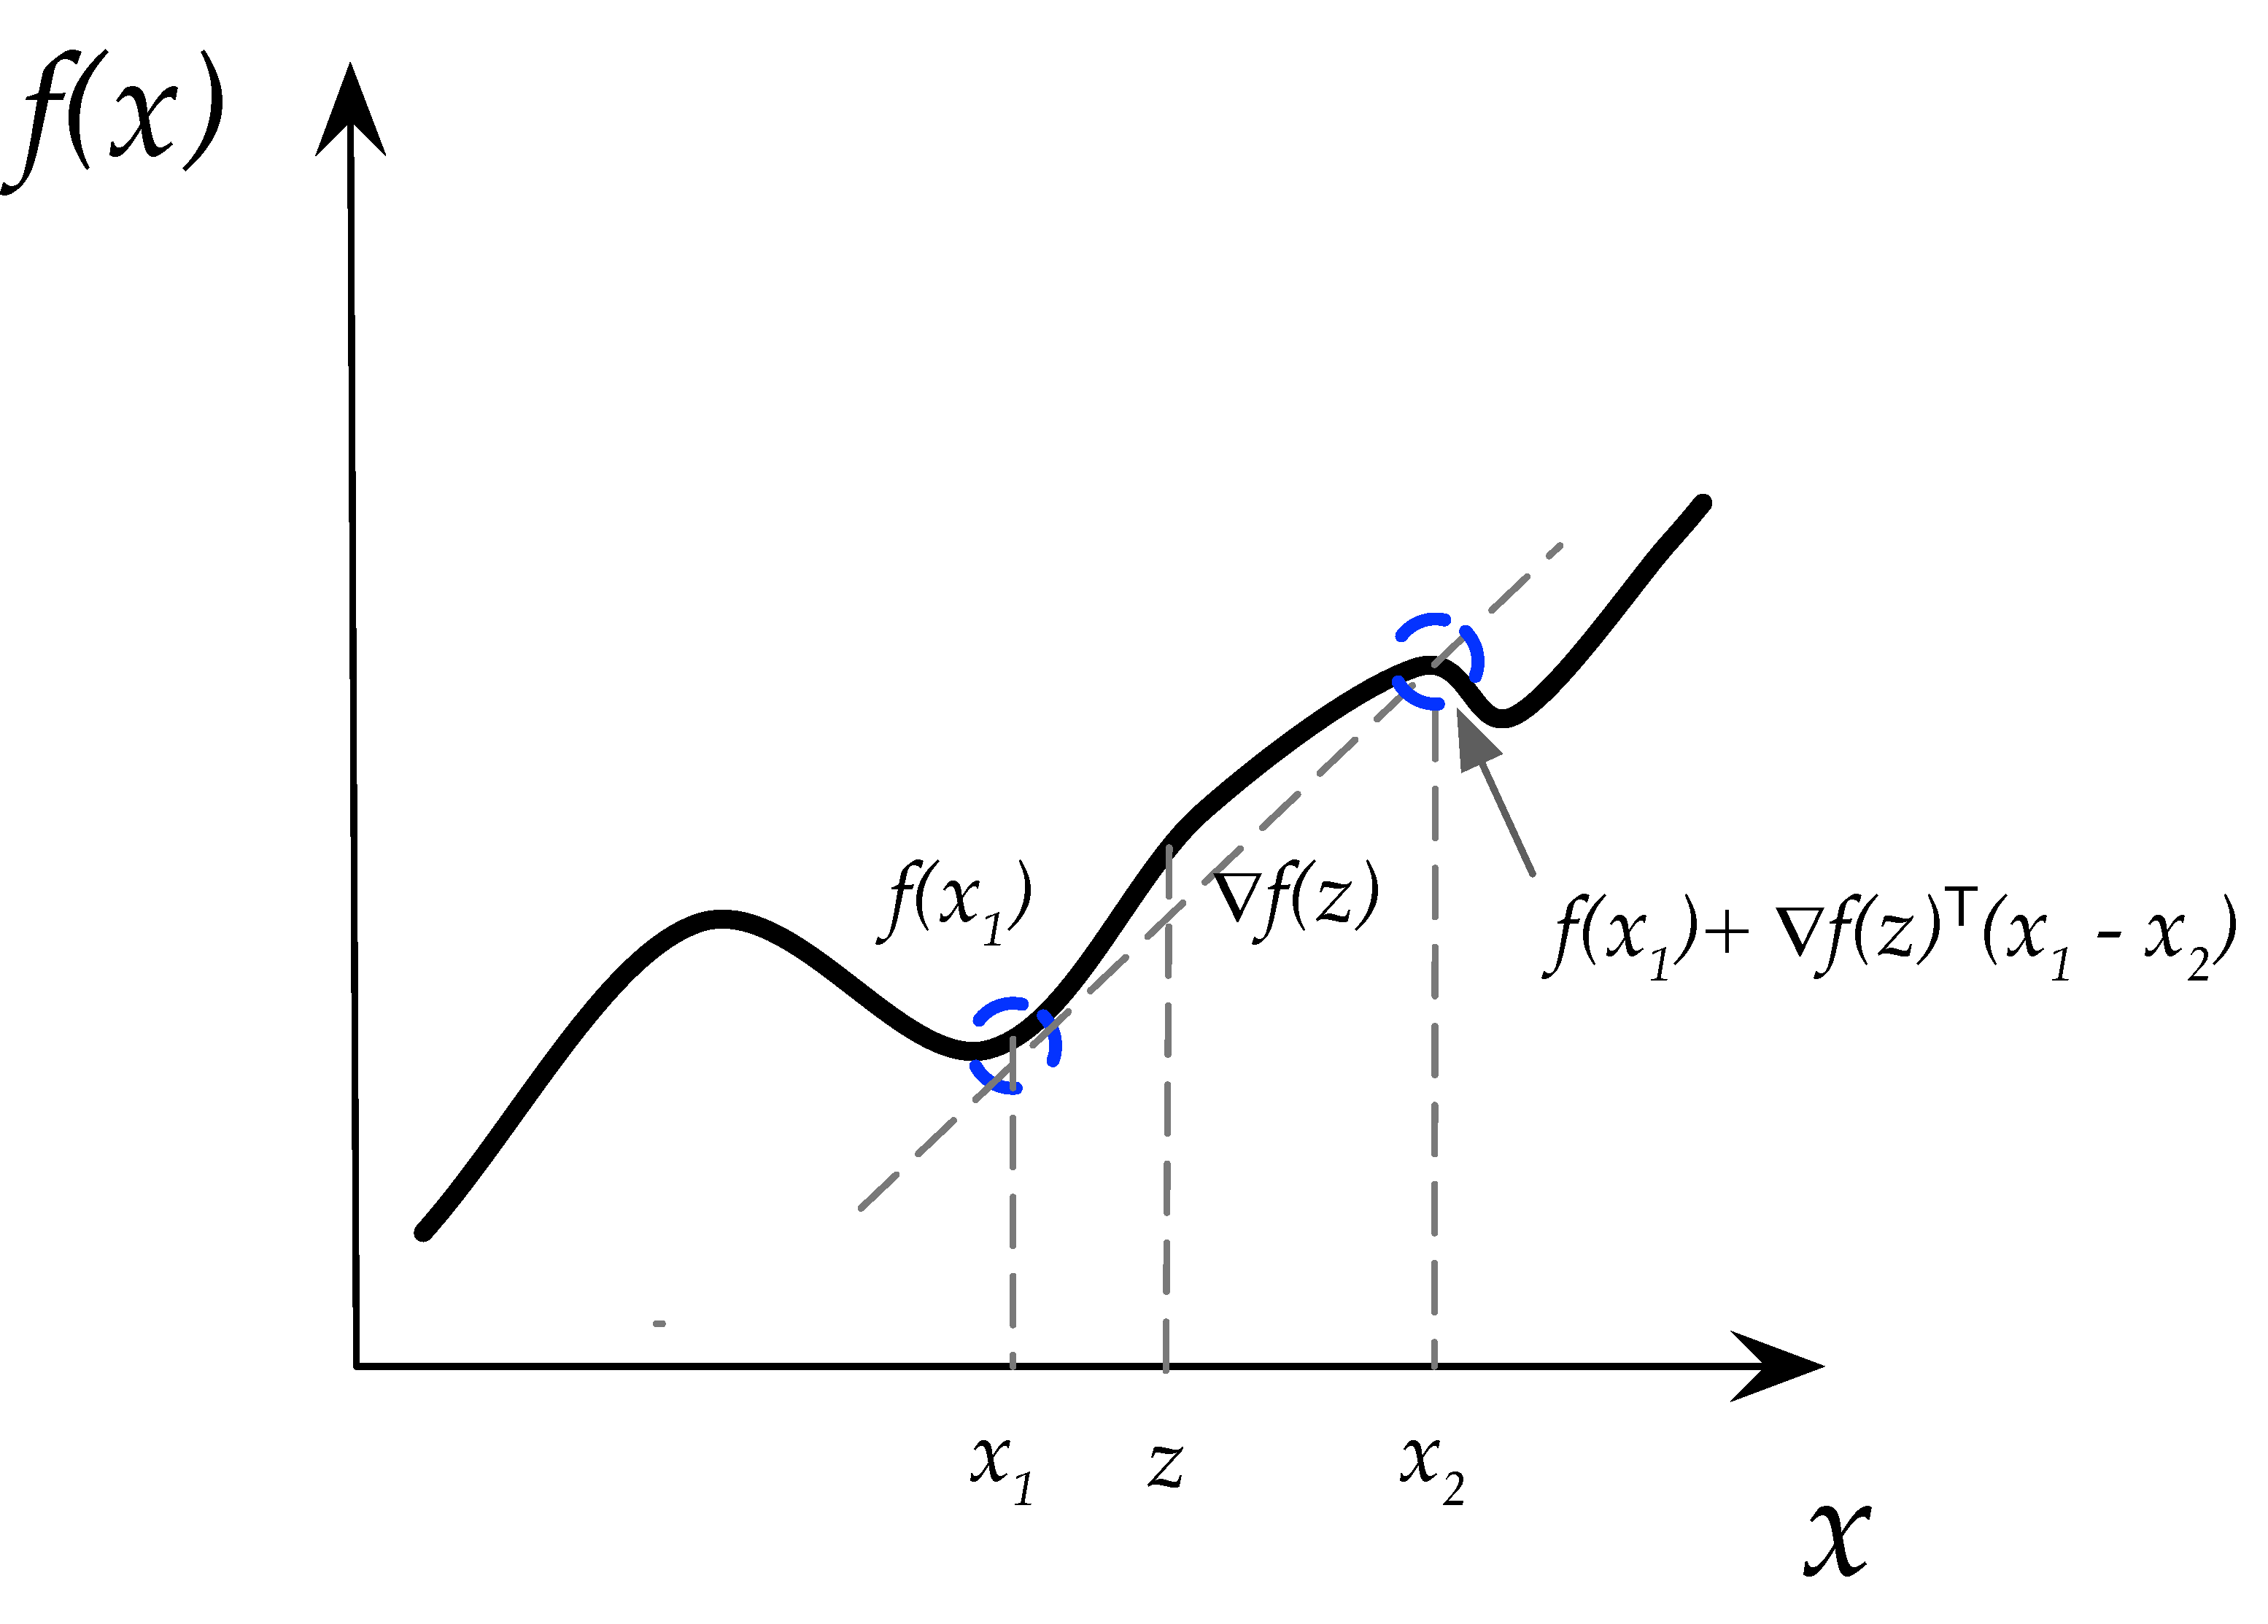
\includegraphics[trim = 0mm 0mm 0mm 0mm, height=60mm]{fig/lec8_taylor2.pdf}
%                 \end{minipage}
%                 \caption{Depiction of first-order Taylor expansion.
%                   \todo{improve this plot}
%                 }\label{fig:taylor}
%               \end{figure}

 \begin{figure}[h]
  \centering
  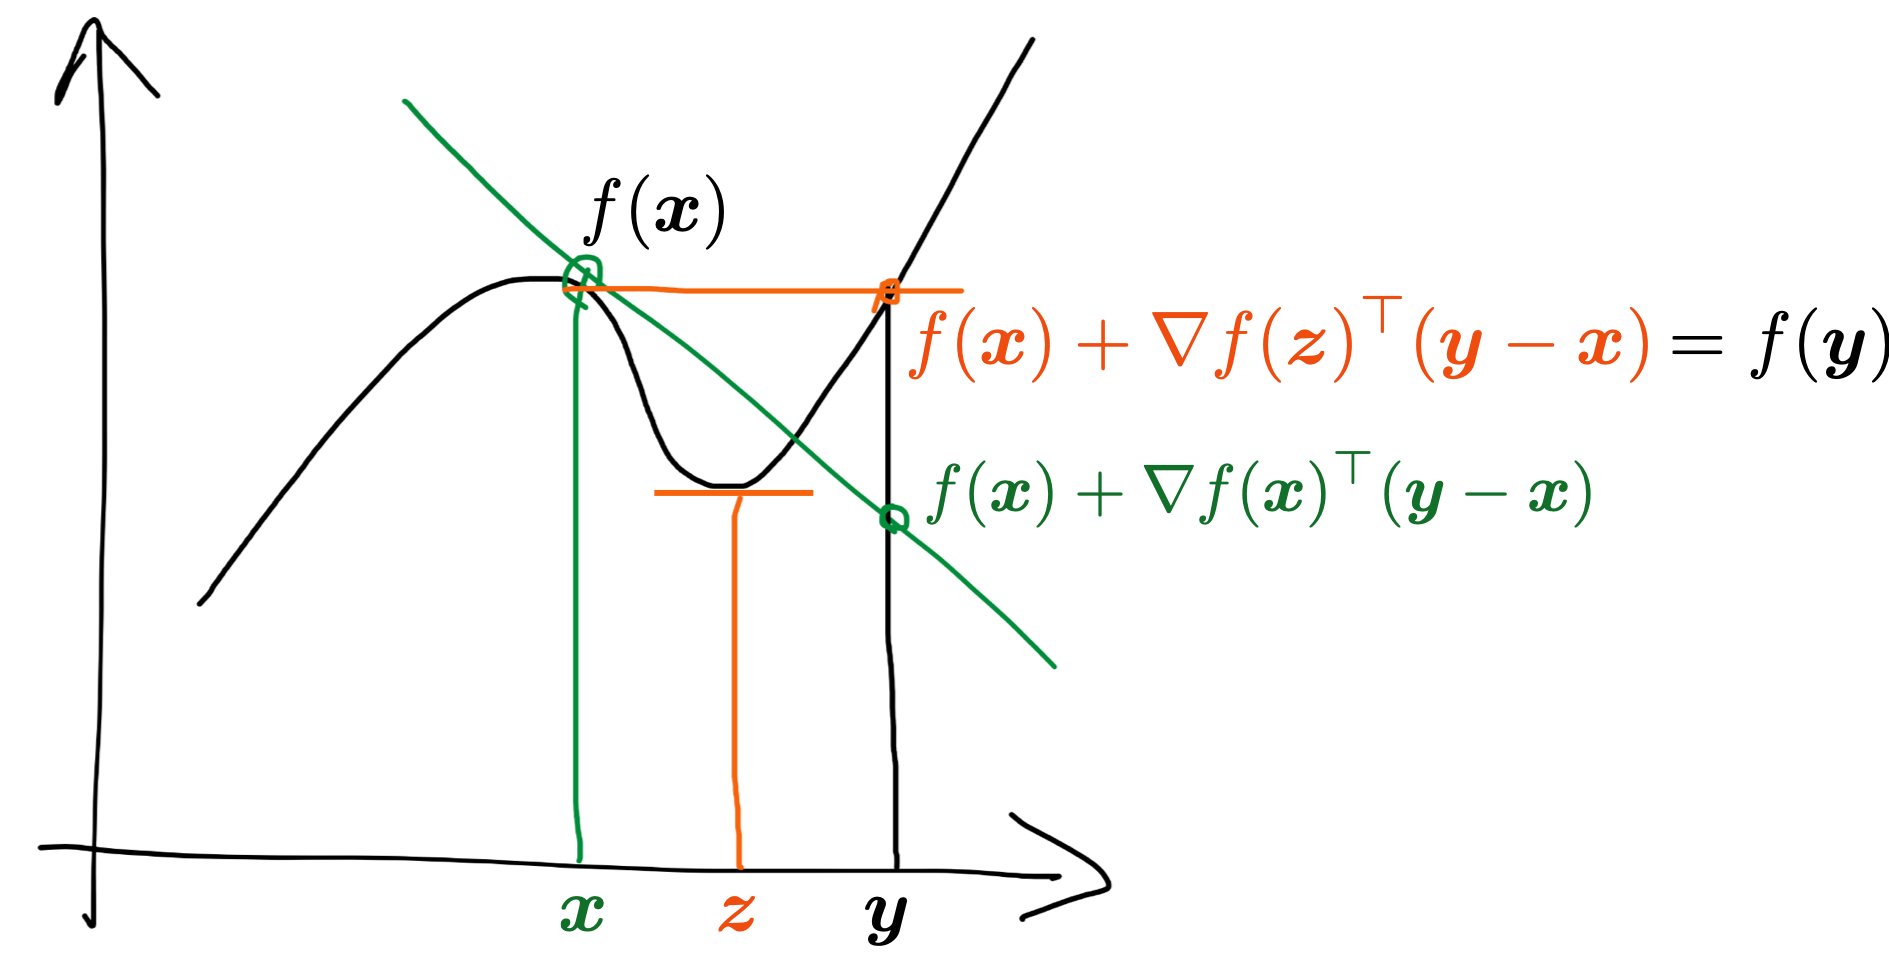
\includegraphics[width=0.4\textwidth]{fig/lecture2_taylor-1st-order-remainder.png}
\caption{The convex function $f(\yy)$ sits above the linear function
  in $\yy$ given by
  ${f(\xx) + \grad f(\xx)^\trp  (\yy-\xx)}$.}
\label{fig:nonjointconvex}
\end{figure}
% LATEXIT NOTES
% f(\boldsymbol{x}) + \mathbf{\nabla} f(\boldsymbol{x})^{\top} (\boldsymbol{y}-\boldsymbol{x})
%

\subsection{Directional Derivatives}

\boxdef{
  Let $f:S \rightarrow \R$
  %where $S \subseteq \R^n$,
  be a function differentiable at $\xx\in S$ and let us consider $\dd\in\R^n$. We define the \textbf{derivative of $f$ at $\xx$ in direction $\dd$} as:
    \begin{displaymath}
        \D{f(\xx)}{\dd} = \lim_{\lambda\rightarrow \veczero}\frac{f(\xx+\lambda \dd)-f(\xx)}{\lambda}
    \end{displaymath}
  }


\begin{proposition}\label{prp:directional}
$\D{f(\xx)}{\dd} = \grad f (\xx)^\trp  \dd$.
\end{proposition}

\begin{proof}
    Using the first order expansion of $f$ at $\xx$:
    \begin{displaymath}
        f(\xx+\lambda \dd) = f(\xx) + \grad f(\xx)^\trp (\lambda \dd) +o(\norm{\lambda \dd}_2)
    \end{displaymath}
    hence, dividing by $\lambda$ (and noticing that $\|\lambda \dd\|_2 = \lambda \norm{ \dd}_2$):
    \begin{displaymath}
        \frac{f(\xx+\lambda \dd)-f(\xx)}{\lambda} = \grad f(\xx)^\trp  \dd + o(\lambda  \norm{ \dd}_2)
    \end{displaymath}
    letting $\lambda$ go to $0$ concludes the proof.
\end{proof}


%\textbf{Example} What is the direction in which $f$ changes the most rapidly? We want to find $d^*\in\arg\max_{\|d\| = 1} f'(x,d) = \grad f(x)^\trp  d$.

%From the Cauchy-Schwarz inequality we get $\grad f(x)^\trp  d\leq \|\grad f(x)\|\|d\|$ with equality when $d = \lambda \grad f(x),\;\lambda\in\R$. Since $\|d\|=1$ this gives:
%\begin{displaymath}
 %   d = \pm\frac{\grad f(x)}{\|\grad f(x)\|}
%\end{displaymath}

\subsection{Lower Bounding Convex Functions with Affine Functions}
In order to prove the characterization of convex functions in the next
section we will need the following lemma.  This lemma says that any
differentiable convex function can be lower bounded by an affine function.


\begin{figure}[h]
  \centering
  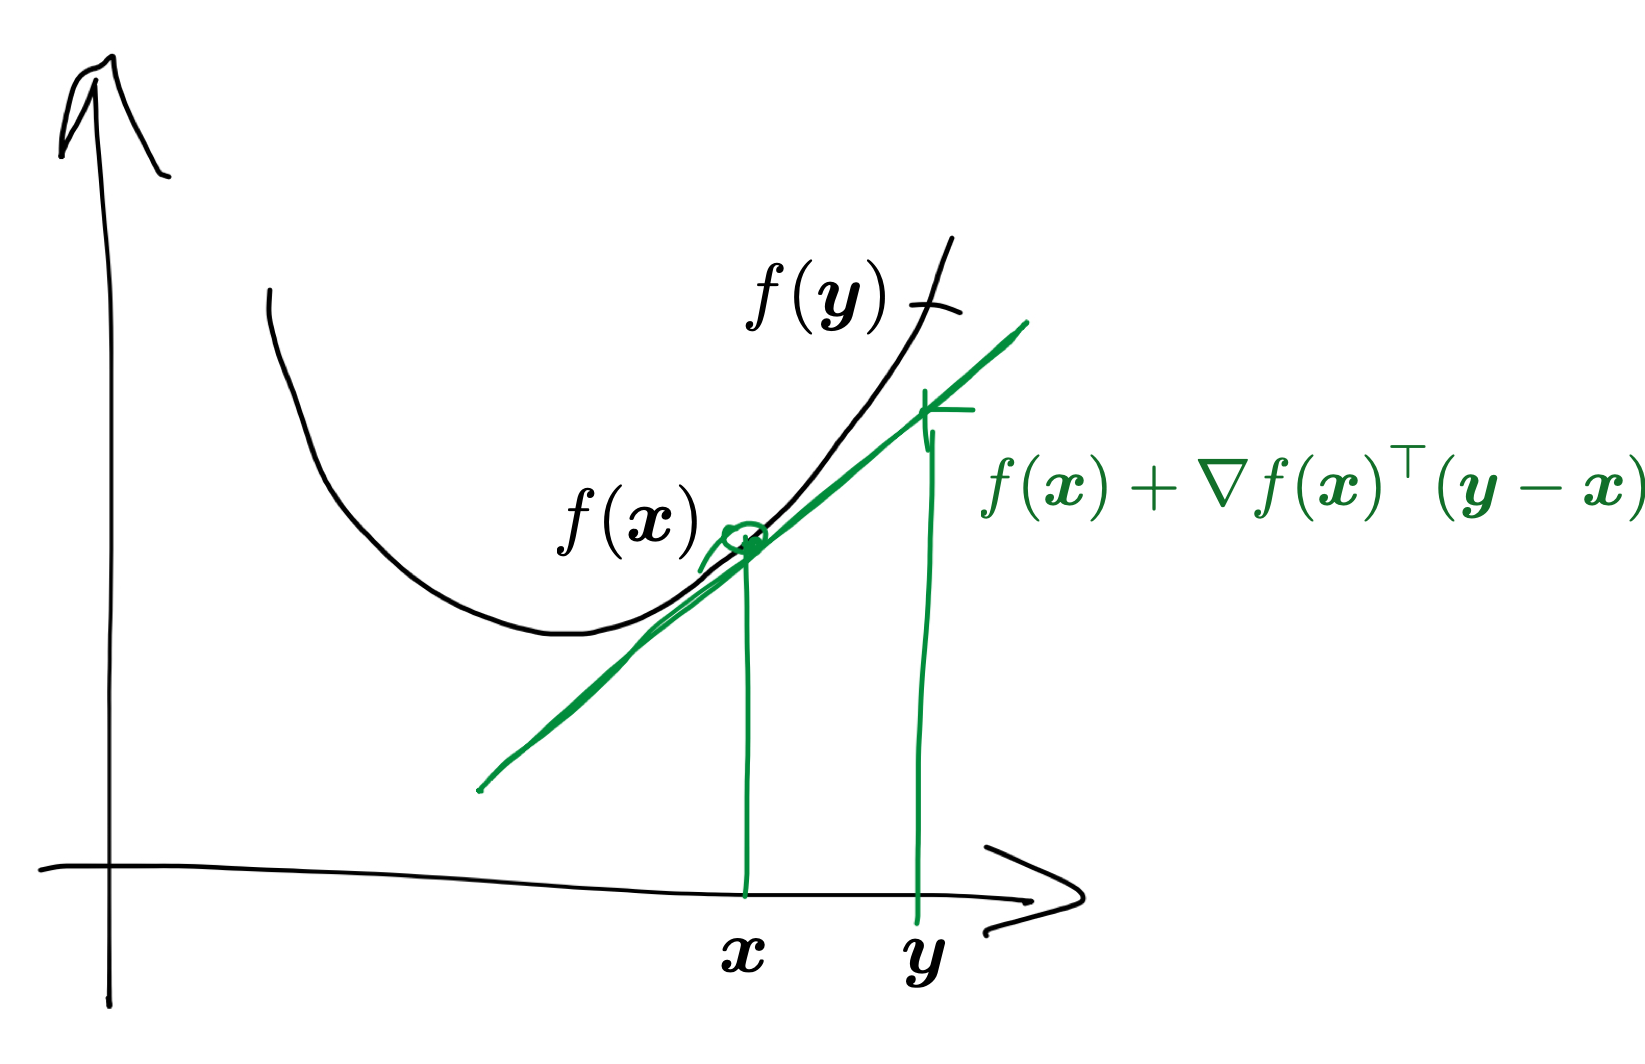
\includegraphics[width=0.4\textwidth]{fig/lecture2_convex-linear-lb.png}
\caption{The convex function $f(\yy)$ sits above the linear function
  in $\yy$ given by
  ${f(\xx) + \grad f(\xx)^\trp  (\yy-\xx)}$.}
\label{fig:nonjointconvex}
\end{figure}
% LATEXIT NOTES
% f(\boldsymbol{x}) + \mathbf{\nabla} f(\boldsymbol{x})^{\top} (\boldsymbol{y}-\boldsymbol{x})
%

\begin{theorem}\label{thm:convexlb}
Let  $S$ be an open convex subset of $\mathbb{R}^n$, and
let $f:S\to \mathbb{R}$ be a  differentiable function.
Then, $f$ is convex if and only if for any $\xx,\yy \in S$ we have that $f(\yy) \geq f(\xx) + \grad f(\xx)^\trp  (\yy-\xx)$.
\end{theorem}

\begin{proof}

  [$\implies$] Assume $f$ is convex, then for all $\mathbf{x,y} \in S$
  and $\theta \in [0,1]$, if we let $\mathbf z = \theta \yy +
  (1-\theta)\xx$, we have that
  \[
    f(\mathbf z) = f((1-\theta)\xx + \theta \yy) \leq
    (1-\theta)f(\xx) + \theta f(\yy)
    \]
    and therefore by subtracting $f(\xx)$ from both sides we get:
\begin{align*}
f\left (\xx + \theta (\yy -\xx)   \right) - f(\xx)
& \leq \theta f(\yy) + (1-\theta)f(\xx) - f(\xx) \\
  & = \theta f(\yy) - \theta f(\xx).
\end{align*}
%
% \begin{align*}
% f\left (\xx + \theta (\yy -\xx)   \right) - f(\xx)
% & = f\left (\theta \yy + (1-\theta)\xx   \right) - f(\xx) \\
% & = f(\mathbf z) - f(\xx) \\
% & \leq \theta f(\yy) + (1-\theta)f(\xx) - f(\xx) \\
% & = \theta f(\yy) - \theta f(\xx).
% \end{align*}
%
Thus we get that (for $\theta > 0$):
$$\frac{f\left (\xx + \theta (\yy -\xx)   \right) - f(\xx)}{\theta} \leq  f(\yy) -  f(\xx)$$

Applying Proposition~\ref{prp:directional} with $\dd =\xx - \yy$ we have that: %$\grad f(\xx)^\trp \mathbf{d} = \lim_{\theta \to 0^{+}} \frac{f(\xx + \theta \mathbf{d}) - f(\xx)}{\theta}$ and therefore:
%
$$\grad f(\xx)^\trp (\yy-\xx) = \lim_{\theta \to 0^{+}} \frac{f(\xx + \theta (\yy - \xx)) - f(\xx)}{\theta} \leq f(\yy) - f(\xx).$$
%
[$\impliedby$] Assume that $f(\yy) \geq f(\xx) + \grad f(\xx)^\trp  (\yy-\xx)$ for all $\mathbf{x,y} \in S$ and show that $f$ is convex.  Let $\mathbf{x,y} \in S$ and $\mathbf z = \theta \yy+(1-\theta)\xx$.  By our assumption we have that:
%
\begin{align}
f(\yy) \geq f(\zz) + \grad f(\zz)^\trp (\yy - \mathbf z) \label{eq:y}  \\
f(\xx) \geq f(\zz) + \grad f(\zz)^\trp (\xx - \mathbf z) \label{eq:x}
\end{align}
%
Observe that $\yy-\zz = (1-\theta)(\yy-\xx)$ and $\xx-\zz = \theta
(\yy-\xx)$.
Thus adding
$\theta$ times \eqref{eq:y} to $(1-\theta)$ times \eqref{eq:x} gives
cancellation of the vectors multiplying the gradient, yielding
\begin{align*}
\theta f(\yy) + (1-\theta)f(\xx)  \nonumber
  & \geq  f(\zz) +  \grad f(\zz)^\trp \veczero
  \\
  & =f(\theta \yy+(1-\theta)\xx)
\end{align*}
This is exactly the definition of convexity.
\end{proof}


\section{Conditions for Optimality}
We now want to find necessary and sufficient conditions for local
optimality.

\boxdef{
  Consider a differentiable function $f: S \to \R$.
A point $\xx \in S $ at which $\grad f(\xx) = \veczero$ is called a \textbf{stationary point}.
}
\begin{proposition}
\label{prp:gradatmin}
    If $\xx$ is a local extremum of a differentiable function
    $f:S\rightarrow \R$
    then $\grad f(\xx) = \veczero$.
\end{proposition}

\begin{proof}
    Let us assume that $\xx$ is a local minimum for $f$. Then for all $\dd\in\R^n$, $f(\xx)\leq f(\xx+\lambda \dd)$ for $\lambda$ small enough. Hence:
    \begin{displaymath}
        0\leq f(\xx+\lambda \dd)-f(\xx) = \lambda \grad f(\xx)^\trp  \dd +
        o(\|\lambda \dd\|)
    \end{displaymath}
    dividing by $\lambda>0$ and letting $\lambda\rightarrow 0^+$, we
    obtain $0\leq \grad f(\xx)^\trp  \dd$.
    But, taking $\dd = - \grad f(\xx) $, we get $0\leq -\norm{\grad f(\xx)}_2^2$.
    This implies that $\grad f(\xx) = \veczero$.

    The case where $\xx$ is a local maximum can be dealt with similarly.
  \end{proof}
  \begin{remark}
    For this proposition to hold, it is important that $S$ is
    open.
  \end{remark}

% The above proposition states that a a stationary point can either be a
% minimum, maximum, or a saddle point of the function, and we will see
% in the following section that the Hessian of the function can be used
% to indicate which one exactly.
For convex functions however it turns out that a stationary point
necessarily implies that the function is at its minimum.
Together with the proposition above, this says that for a convex function on
$\R^n$ a point is optimal if and only if it is stationary.

\begin{proposition}
Let $S \subseteq \mathbb{R}^n$ be an open convex set and let $f: S \to \R$ be a
differentiable and convex function.  If $\xx$ is a stationary point then $\xx$ is a global minimum.
\end{proposition}

\begin{proof}
From Theorem~\ref{thm:convexlb} we know that for all $\xx,\yy \in S$ : $f(\yy) \geq f(\xx) + \grad f(\xx)(\yy - \xx)$.
Since $\grad f(\xx) = \veczero$ this implies that $f(\yy) \geq
f(\xx)$.  As this holds for any $\yy \in S$, $\xx$ is a global
minimum.

%
%Using the Taylor expansion of $f$ we know that for any $\yy\in S$ there is some point $\zz \in [\bar{\xx},\yy]$ s.t.:
%$$
%f(\yy) = f(\bar{\xx}) + \grad f(\bar{\xx})(\yy - \bar{\xx}) + \frac{1}{2}(\yy - \bar{\xx}) ^TH_{f}(\zz)(\yy - \bar{\xx}).
%$$
%Since $f$ is convex, the Hessian must be positive semi-definite, and since $\bar{\xx}$ is a stationary point, then $ \grad f(\bar{\xx})(\yy - \bar{\xx})  = 0$.  This leaves us with:
%$$f(\yy) \geq f(\bar{\xx}).$$
%Since this holds for all $\yy \in S$, we have that $\bar{\xx}$ is a global minimum.
\end{proof}




% \FloatBarrier


% \newpage
% \section*{Exercises}
% \begin{itemize}
% \item sufficient conditions for optimality (see below)
% \item taylor theorem remainder form
% \item \url{https://en.wikipedia.org/wiki/Min-max_theorem}
% \item \todo{maybe} pointwise max of convex gives convex
% \item \todo{maybe} joint convex, min over one coord, gives another
%   convex fn
% \item norm equals eigenvalue claim plus counter example. Claim~\ref{clm:symnorm}
% \end{itemize}
% BONUS, GRADED:
% \begin{enumerate}
% \item For each of the following functions answer these questions:
%   \begin{itemize}
%   \item  Is the function convex?
%   \item  \todo{add strongly convex?}
%   \end{itemize}
%   \begin{enumerate}
%   \item $f(x) = \abs{x}^6$ on $x \in \R$
%   \item $f(x) = \abs{x}^{1.5}$ on $x \in \R$
%   \item $f(x) = \exp(x)$ on $x \in \R$
%   \item $f(x) = \exp(x)$ on $x \in (-1,1)$
%   \item $f(x,y) = \sqrt{x+y}$ on $ (x,y)  \in (0,1) \times (0,1)$.
%   \item $f(x,y) = \sqrt{x+y}$ on $ (x,y)  \in (1/2,1) \times (1/2,1)$.
%   \item  $f(x,y) = \sqrt{x^2+y^2}$ on $ (x,y)  \in \R^2$.
%   \item $f(x) = \log(x)$ on $x \in (0,\infty)$
%   \item $f(x) = -\log(x)$ on $x \in (0,\infty)$
%   \item $f(x,y) = \log(\exp(x) + \exp(y))$ on $ (x,y)  \in \R^2$.
%   \end{enumerate}

% \end{enumerate}

% \newpage
% \section*{Background}
% \todo{terminology \& citations}

% \begin{itemize}
% \item \url{https://francisbach.com/chebyshev-polynomials/}
% \item
%   \url{https://sachdevasushant.github.io/courses/15s-cpsc665/notes/linsys.pdf}
%   \begin{itemize}
%   \item starts off well but doesn't get to polynomials
%   \end{itemize}
% \item
%   \url{https://sachdevasushant.github.io/pubs/fast-algos-via-approx-theory.pdf}
% \item spielman
%   \begin{itemize}
%   \item \url{http://www.cs.yale.edu/homes/spielman/561/2012/lect17-12.pdf}
%   \item
%     \url{http://www.cs.yale.edu/homes/spielman/561/2012/lect18-12.pdf}
%   \item let's use these plus...? maybe sushant on the polynomial?
%   \item but we could also use Sushant's monograph?
%   \end{itemize}
% \end{itemize}


% \subsection{Sufficient Condition for Optimality}
% \todo{turn this into an exercise}
% The following theorem, which is a fundamental theorem in real analysis, gives us a sufficient (though not necessary) condition for optimality.  Before stating the theorem, let's first recall the Bolzano-Weierstrass theorem from real analysis (which you will prove in section this week).

% \boxthm{(Bolzano-Weierstrass)
% Every bounded sequence in $\mathbb{R}^n$ has a convergent subsequence.
% }

% Secondly, we recall the boundedness theorem:

% \boxthm{(Boundedness Theorem)
% Let $f:\mathbb{R}^n \to \mathbb{R}$ be a continuous function and $\mathcal{F} \subseteq \mathbb{R}^n$ be nonempty, bounded, and closed.
% Then $f$ is bounded on $\mathcal{F}$.
% }
% %
% \begin{theorem*}[Extreme Value Theorem]
% Let $f:\mathbb{R}^n \to \mathbb{R}$ be a continuous function and $\mathcal{F} \subseteq \mathbb{R}^n$ be nonempty, bounded, and closed.  Then, the optimization problem $\min f(\xx) : \xx \in \mathcal{F}$ has an optimal solution.
% \end{theorem*}


% % \begin{theorem*}[Weierstrass]
% % Let $f:\mathbb{R}^n \to \mathbb{R}$ be a continuous function and $\mathcal{F} \subseteq \mathbb{R}^n$ be nonempty, bounded, and closed.  Then, the optimization problem $\min f(\xx) : \xx \in \mathcal{F}$ has an optimal solution.
% % \end{theorem*}

% \begin{proof}
% Let $\alpha$ be the infimum of $f$ over $\mathcal{F}$ (i.e. the largest value for which any point $\xx \in \mathcal{F}$ respects $f(\xx)\geq \alpha$);
% by the Boundedness Theorem, such a value exists, as $f$ is lower-bounded, and the set of lower bounds has a greatest lower bound, $\alpha$.

% Let
% %
% $$\mathcal{F}_k := \{ \xx \in \mathcal{F}: \alpha \leq f(\xx) \leq \alpha + 2^{-k}\}.$$
% %
% $\mathcal{F}_k$ cannot be empty, since if it were, then $\alpha + 2^{-k}$ would be a strictly greater lower bound on $f$ than $\alpha$.
% For each $k$, let $\xx_k$ be some $\xx \in \mathcal{F}_k$.
% $\setof{\xx_k}_{k = 1}^{\infty}$ is a bounded sequence as
% $\mathcal{F}_k \subseteq \mathcal{F}$, so the Bolzano-Weierstrass
% theorem we know that there is a convergent subsequence,
% $\setof{\yy_k}_{k = 1}^{\infty}$, with limit $\bar{\yy}$.
% Because the set is closed, $\bar{\yy} \in \mathcal{F}$.
% By continuity $f(\bar{\yy}) = \lim_{k \to \infty} f(\yy_k)$, while by
% construction, $\lim_{k \to \infty} f(\yy_k) = \alpha$.

% Thus, the optimal solution is $\bar{\yy}$.
% \end{proof}


% \newpage





%\end{document}

%%% Local Variables:
%%% mode: latex
%%% TeX-master: "main"
%%% TeX-engine: luatex
%%% End: